\documentclass[tikz,border=4pt]{standalone}
\usepackage{amsmath,amssymb}
\usepackage{mathptmx}
\usepackage{pgfplots}
\pgfplotsset{compat=1.18}
\usetikzlibrary{arrows.meta,positioning,calc,decorations.pathmorphing,backgrounds,fit,shapes.geometric}
\begin{document}
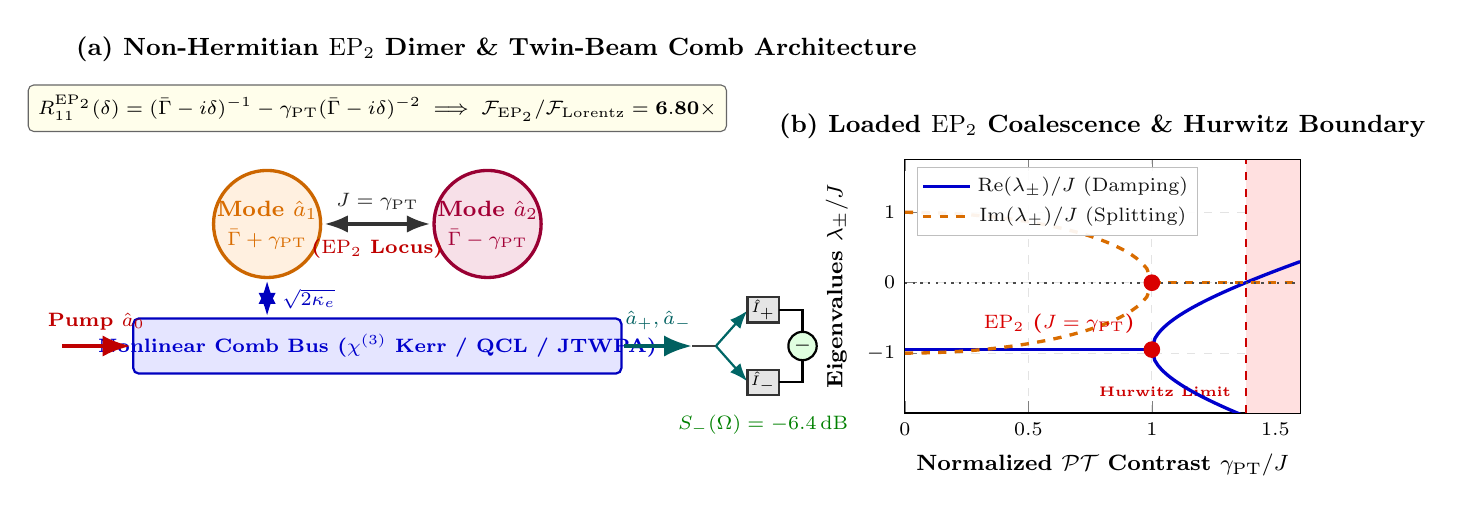
\begin{tikzpicture}[font=\small, >=Latex]
  % ==================== PANEL (a): Architecture Schematic ====================
  \begin{scope}[shift={(0,0)}]
    \node[anchor=north west, font=\bfseries\small] at (-0.6, 5.05) {(a) Non-Hermitian $\mathrm{EP}_2$ Dimer \& Twin-Beam Comb Architecture};

    % Primary Bus Waveguide (QCL Ridge / Si3N4 Bus / JTWPA Line)
    \fill[blue!10, draw=blue!75!black, thick, rounded corners=2pt] (0.25, 0.65) rectangle (6.45, 1.35);
    \node[font=\scriptsize\bfseries, blue!80!black] at (3.35, 1.0) {Nonlinear Comb Bus ($\chi^{(3)}$ Kerr / QCL / JTWPA)};

    % Input Pump and Output Comb Arrows
    \draw[->, ultra thick, red!75!black] (-0.65, 1.0) -- (0.22, 1.0);
    \node[anchor=south, font=\scriptsize\bfseries, red!75!black] at (-0.22, 1.08) {Pump $\hat{a}_0$};
    \draw[->, ultra thick, teal!75!black] (6.48, 1.0) -- (7.35, 1.0);
    \node[anchor=south, font=\scriptsize\bfseries, teal!75!black] at (6.92, 1.08) {$\hat{a}_+, \hat{a}_-$};

    % Resonator 1 (Lossy / Bus-Loaded Mode a1)
    \fill[orange!12, draw=orange!80!black, very thick] (1.95, 2.55) circle (0.68cm);
    \node[font=\footnotesize\bfseries, orange!85!black] at (1.95, 2.72) {Mode $\hat{a}_1$};
    \node[font=\scriptsize, orange!85!black] at (1.95, 2.36) {$\bar{\Gamma} + \gamma_{\mathrm{PT}}$};

    % Resonator 2 (Regenerative / Auxiliary Gain Mode a2)
    \fill[purple!12, draw=purple!80!black, very thick] (4.75, 2.55) circle (0.68cm);
    \node[font=\footnotesize\bfseries, purple!85!black] at (4.75, 2.72) {Mode $\hat{a}_2$};
    \node[font=\scriptsize, purple!85!black] at (4.75, 2.36) {$\bar{\Gamma} - \gamma_{\mathrm{PT}}$};

    % Evanescent Coupling Bus <-> a1 (kappa_e)
    \draw[<->, very thick, blue!75!black] (1.95, 1.38) -- (1.95, 1.83);
    \node[anchor=west, font=\scriptsize\bfseries, blue!75!black] at (2.02, 1.60) {$\sqrt{2\kappa_e}$};

    % Inter-Resonator Coupling a1 <-> a2 (J = gamma_PT)
    \draw[<->, very thick, black!80] (2.68, 2.55) -- (4.02, 2.55);
    \node[anchor=south, font=\scriptsize\bfseries, black!85] at (3.35, 2.60) {$J = \gamma_{\mathrm{PT}}$};
    \node[anchor=north, font=\scriptsize\bfseries, red!75!black] at (3.35, 2.48) {($\mathrm{EP}_2$ Locus)};

    % Top Banner Box for Double-Pole Resolvent Identity
    \node[draw=black!60, fill=yellow!8, rounded corners=2pt, inner sep=3.5pt, font=\scriptsize] at (3.35, 4.02)
      {$R_{11}^{\mathrm{EP}_2}(\delta) = (\bar{\Gamma} - i\delta)^{-1} - \gamma_{\mathrm{PT}}(\bar{\Gamma} - i\delta)^{-2} \implies \mathcal{F}_{\mathrm{EP}_2}/\mathcal{F}_{\mathrm{Lorentz}} = \mathbf{6.80\times}$};

    % Balanced Twin-Beam Detector Readout on Right
    \draw[thick, black!75] (7.35, 1.0) -- (7.65, 1.0);
    \draw[->, thick, teal!80!black] (7.65, 1.0) -- (8.05, 1.45);
    \draw[->, thick, teal!80!black] (7.65, 1.0) -- (8.05, 0.55);
    \fill[gray!20, draw=black!80, thick] (8.05, 1.30) rectangle (8.45, 1.62);
    \fill[gray!20, draw=black!80, thick] (8.05, 0.38) rectangle (8.45, 0.70);
    \node[font=\tiny\bfseries] at (8.25, 1.46) {$\hat{I}_+$};
    \node[font=\tiny\bfseries] at (8.25, 0.54) {$\hat{I}_-$};
    \draw[thick] (8.45, 1.46) -| (8.75, 1.18);
    \draw[thick] (8.45, 0.54) -| (8.75, 0.82);
    \draw[thick, fill=green!12] (8.75, 1.0) circle (0.18cm);
    \node[font=\scriptsize\bfseries] at (8.75, 1.0) {$-$};
    \node[anchor=north, font=\scriptsize\bfseries, green!50!black] at (8.25, 0.25) {$S_-(\Omega) = -6.4\,\mathrm{dB}$};
  \end{scope}

  % ==================== PANEL (b): Eigenvalue Coalescence ====================
  \begin{scope}[shift={(10.05, 0.15)}]
    \begin{axis}[
      width=6.6cm,
      height=4.8cm,
      xlabel={Normalized $\mathcal{PT}$ Contrast $\gamma_{\mathrm{PT}}/J$},
      ylabel={Eigenvalues $\lambda_\pm / J$},
      xmin=0.0, xmax=1.60,
      ymin=-1.85, ymax=1.75,
      grid=both,
      grid style={gray!22, dashed},
      tick label style={font=\scriptsize},
      label style={font=\footnotesize\bfseries},
      title={\textbf{(b) Loaded $\mathrm{EP}_2$ Coalescence \& Hurwitz Boundary}},
      title style={font=\small, yshift=-2pt},
      legend style={at={(0.03,0.97)}, anchor=north west, font=\scriptsize, fill=white, fill opacity=0.92, draw=gray!50, inner sep=1.5pt},
    ]
      % Shaded Hurwitz-unstable region (gamma_PT/J > sqrt(1 + (Gamma_bar/J)^2) = 1.38)
      \addplot[fill=red!12, draw=none, forget plot] coordinates {(1.38, -1.85) (1.60, -1.85) (1.60, 1.75) (1.38, 1.75)};
      \draw[dashed, red!80!black, thick] (axis cs:1.38,-1.85) -- (axis cs:1.38,1.75);
      \node[anchor=east, font=\tiny\bfseries, red!80!black] at (axis cs:1.36, -1.55) {Hurwitz Limit};

      % Real parts Re(lambda_pm)/J with Gamma_bar/J = 0.95
      \addplot[blue!80!black, very thick, domain=0:1.0, samples=40] {-0.95};
      \addlegendentry{$\mathrm{Re}(\lambda_\pm)/J$ (Damping)}
      \addplot[blue!80!black, very thick, domain=1.0:1.6, samples=50, forget plot] {-0.95 + sqrt(x^2 - 1.0)};
      \addplot[blue!80!black, very thick, domain=1.0:1.6, samples=50, forget plot] {-0.95 - sqrt(x^2 - 1.0)};

      % Imaginary parts Im(lambda_pm)/J
      \addplot[orange!85!black, very thick, dashed, domain=0:1.0, samples=50] {sqrt(1.0 - x^2)};
      \addlegendentry{$\mathrm{Im}(\lambda_\pm)/J$ (Splitting)}
      \addplot[orange!85!black, very thick, dashed, domain=0:1.0, samples=50, forget plot] {-sqrt(1.0 - x^2)};
      \addplot[orange!85!black, very thick, dashed, domain=1.0:1.6, samples=20, forget plot] {0.0};

      % Zero line (self-oscillation threshold Re(lambda_+) = 0)
      \draw[dotted, black!70, thick] (axis cs:0.0, 0.0) -- (axis cs:1.60, 0.0);

      % Mark EP2 Point at gamma_PT/J = 1.0
      \addplot[only marks, mark=*, mark size=2.8pt, red!85!black, forget plot] coordinates {(1.0, -0.95) (1.0, 0.0)};
      \node[anchor=south east, font=\scriptsize\bfseries, red!85!black] at (axis cs:0.97, -0.86) {$\mathrm{EP}_2$ ($J=\gamma_{\mathrm{PT}}$)};
    \end{axis}
  \end{scope}
\end{tikzpicture}
\end{document}
